\chapter{ روش پیشنهادی }
\section{مقدمه}

شناسایی بی‌درنگ چهره در محیط بدون محدودیت و با دقت بالا با چالش‌های بسیاری همراه است. همچنین دقت بالا و زمان پردازش سریع باهم در تقابل هستند. علاوه بر این‌ها، فرض ‌کمبود داده آموزشی نیز چالش بزرگی محسوب می‌شود. بنابراین در این فصل تلاش می‌کنیم تا روشی برای تشخیص دقیق‌تر و بی‌درنگ چهره توسط شبکه عصبی عمیق در تصاویر بدون محدودیت پیشنهاد دهیم. در ابتدا مرحله پیش پردازش شرح داده می‌شود. در قسمت بعد، رویكرد استفاده شده مبتنی بر شبكه‌های پیچشی به منظور استخراج ویژگی از تصاویر چهره شرح داده خواهد شد. نمای کلی روش ارائه شده در شكل \ref{image4-1} خلاصه شده است كه در ادامه هر یک تشریح خواهد شد.

\begin{figure}[h]
	\label{image4-1}
	\centering
  	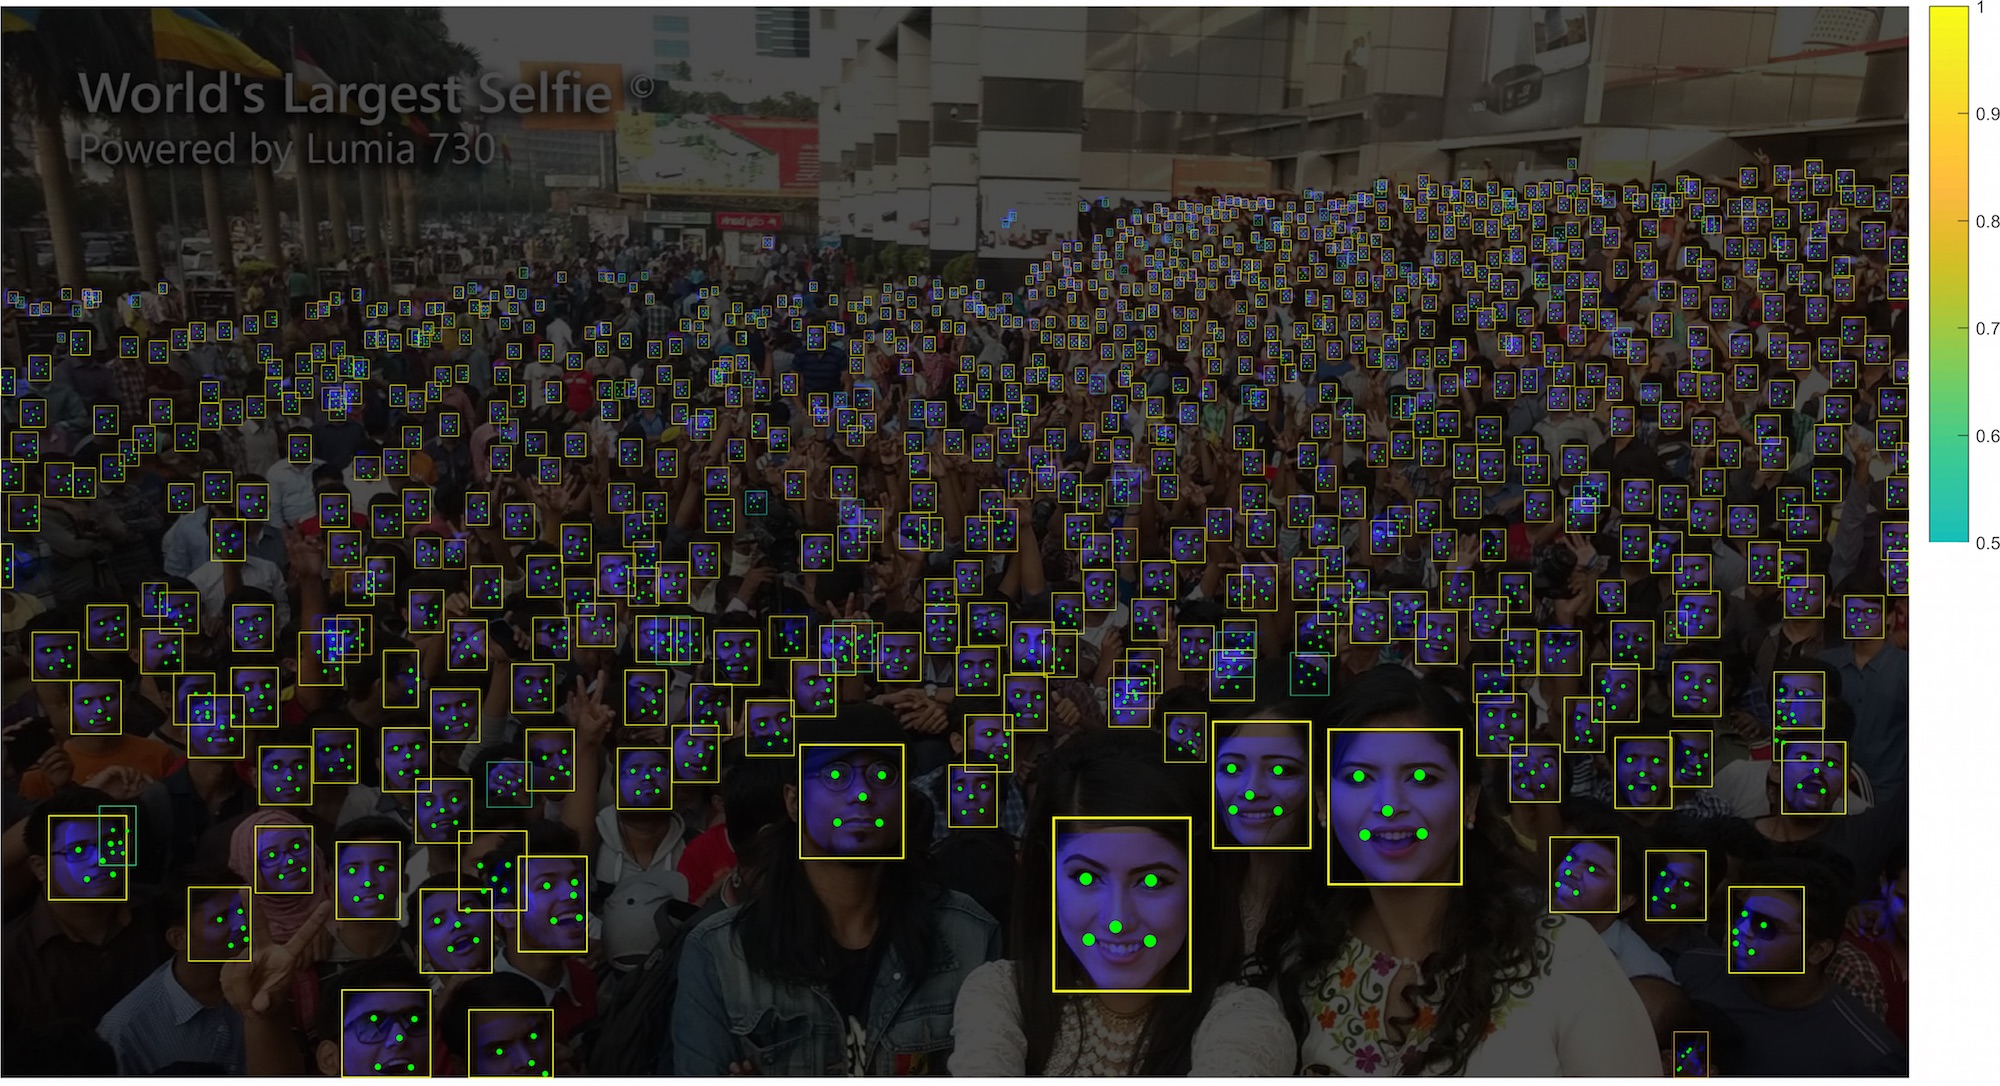
\includegraphics[width=1.0\textwidth]{image4-1}
  	\caption{نمای کلی از روش پیشنهادی.}
\end{figure}

\section{پیش پردازش}
بیشتر الگوریتم‌ها‌ی شناسایی چهره نیاز به اعمال پیش‌پردازش‌هایی بر روی تصویر ورودی دارند. در این روش، پیش‌پردازش شامل همسان سازی بافت‌نگار به منظور افزایش تباین، یافتن چهره و تراز کردن تصویر می‌باشد. در ادامه به شرح مراحل پیش‌پردازش می‌پردازیم.
\subsection{همسان سازی بافت‌نگار}
یکی از روش‌های بهبود تصویر، افزایش تباین تصویر است. برای بهبود تباین، می‌توان از تکنیک یکنواخت‌سازی بافت‌نگار تصویر استفاده کرد. این عمل باعث افزایش تباین تصویر  می‌شود که به معنای بهبود کیفیت تصویر و افزایش دقت پردازش های بعدی است. در سال ۲۰۱۸ چو و همکاران \cite{s18092995} یک الگوریتم بهبود تباین مبتنی بر یکنواخت‌سازی بافت‌نگار ارائه دادند که در این بخش از آن استفاده می‌کنیم.

\subsection{یافتن چهره}
برای یافتن چهره‌ها در تصویر از الگوریتم RetinaFace که توسط \lr{Deng} و همکاران \cite{deng2019retinaface} در سال ۲۰۱۹معرفی شده است استفاده می‌کنیم. ما برای رسیدن به خروجی بی‌درنگ، این روش را بر روی معماری \lr{MobileNetV3} پیاده سازی کرده و آموزش دادیم. نمونه‌ای از خروجی این روش را در شکل \ref{image4-3} مشاهده می‌کنید. 

\begin{figure}[h]
\centering
  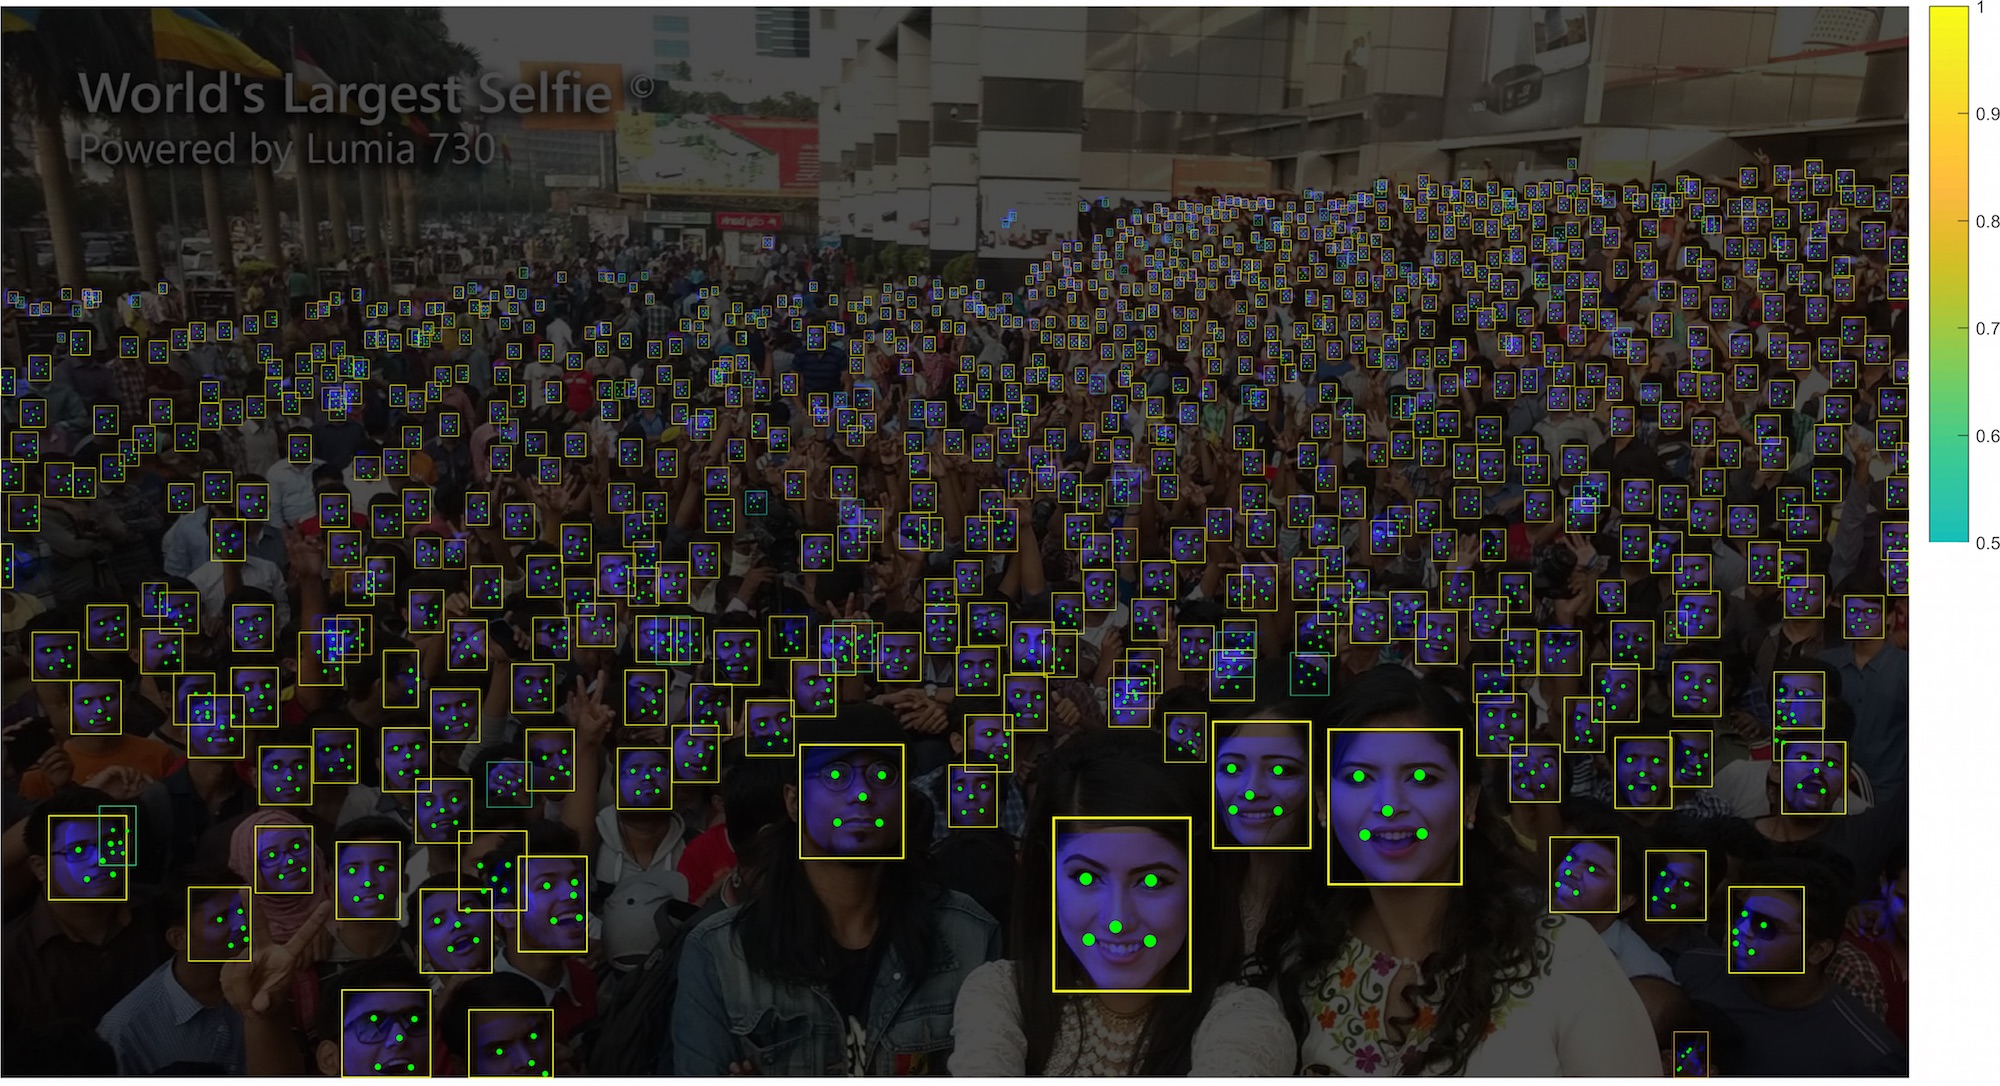
\includegraphics[width=1.0\textwidth]{image4-3}
  \caption{نمونه از خروجی الگوریتم یافتن چهره retina \cite{deng2019retinaface}.}
  \label{image4-3}
\end{figure}

\subsection{تراز کردن تصویر}
در ادامه روند پیش‌پردازش، نوبت به تراز کردن تصویر چهره \LTRfootnote{Face Alignment} می‌رسد. پس از یافتن چهره، به تصویر ورودی مناسب شبکه نزدیک‌تر می‌شویم، اما پس از تراز کردن تصویر جهت آموزش شبکه، بهبود دقت نهایی مشهود است.  بدین منظور با استفاده از یک تبدیل غیرخطی، تصویر چهره را به گونه ای می‌چرخانیم که چشم‌ها در راستای خط افقی قرار بگیرند. روش‌های کلی برای تشخیص چهره از زاویه‌ی روبه‌رو به خوبی عمل می‌کنند اما مقاومت این روش‌ها در مقابل تغییرات زاویه مناسب نیست، به این علت که ویژگی‌های ظاهری با تغییرات زاویه بسیار تغییر پذیر هستند. با تراز کردن تصویر چهره پیش از اعمال طبقه‌بند می‌توان این مشکل را بهبود داد. در طول ‌تراز کردن تصویر، نقاط خاصی از تصویر (مانند نقطه‌ وسط دو چشم و نقاط دو طرف دهان) در نظر گرفته می‌شود و به مختصات مشخصی منتقل می‌شوند. برای این منظور از ۵ نقطه ویژه استخراج شده در مرحله یافتن چهره توسط الگوریتم retina استفاده می‌کنیم. نتیجه اعمال این فرآیند را در شکل \ref{image4-4} مشاهده می‌کنید. در نهایت تصاویر چهره با اندازه $112 \times 112$ پیکسل ذخیره می‌گردند تا در مرحله آموزش شبکه، مورد استفاده قرار گیرند.
\begin{figure}[h]
\centering
  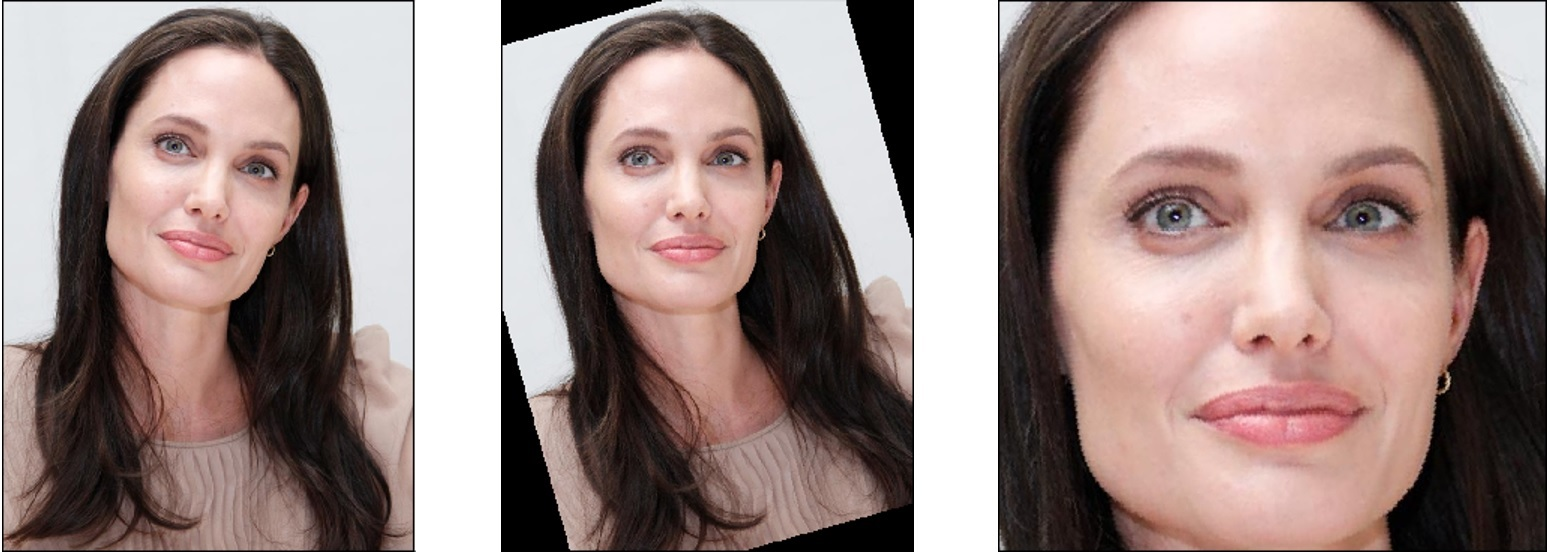
\includegraphics[width=1.0\textwidth]{image4-4}
  \caption{به منظور افزایش دقت شبکه، پس از یافتن چهره باید آن را تراز کرد.}
  \label{image4-4}
\end{figure}

\section{دسته بندی}
روش پیشنهادی برای تشخیص بی‌درنگ چهره در محیط های بدون محدودیت، یک الگوریتم مبتنی بر شبکه های پیچشی می‌باشد. این فرایند را می توان به صورت یک مسئله بهینه سازی فرموله کرد که در ادامه به بخش های مختلف آن می پردازیم.

\subsection{مدل پیشنهادی پایه}
در این بخش ابتدا باید معماری مناسب شبکه پایه برای مسئله را به دست آوریم. با بررسی شبکه‌های متداول و مقایسه دقت و زمان پاسخگویی آن‌ها به کمک یادگیری انتقال، به این نتیجه می‌رسیم که شبکه \lr{MobileNetV3} دارای چگالی دقت بالاتری در مقایسه با شبکه های دیگر می‌باشد و نسبت دقت دسته بندی به تعداد پارامترهای شبکه در آن‌ بیشتر می‌باشد. بنابرین می‌توان سرعت اجرای مناسب و همچنین دقت مناسب را از این شبکه‌ انتظار داشت. از نتایج در می‌یابیم که بهترین معماری شبکه برای مسئله ما معماری \lr{MobileNetV3} است. نتایج آزمایش در جدول \ref{table4-1} آمده است. آزمایش‌هایی بر روی معماری‌های مطرح دیگر نیز انجام شد که به علت ضعیف بودن نتایج یا بالا بودن زمان پاسخ دهی در جدول درج نشده اند.

\begin{table}[ht]
\label{table4-1}
\begin{center}
\caption{مقایسه و ‌ارزیابی برخی از معماری شبکه های رایج در زمینه بینایی ماشین}
\resizebox{\textwidth}{!}
{
\begin{tabular}{|c|c|c|c|}
\hline 
نام شبکه & تعداد پارامترها & دقت بر روی مجموعه داده LFW
\\
\hline 
\lr{MobileNetV2} & \lr{3.53M} & \lr{93.50}
\\
\hline
\lr{MobileNetV3} & \lr{2.5M} & \lr{95.8} 	 
\\
\hline
\lr{SqueezeNet} & \lr{1.25M} & \lr{89.2}
\\
\hline 
\lr{NASNetMobile} & \lr{5.32M} & \lr{90.60}
\\
\hline
\lr{EfficientNetB0} & \lr{5.3M} & \lr{85.50}
\\
\hline
\end{tabular}
}
\end{center} 
\end{table}

\noindent
تشخیص چهره به دلیل وجود پیكسل‌های مشابه از نظر شدت روشنایی در تصویر بسیار چالش برانگیز بوده است. از آنجا كه عملیات كانولوشن به پنجره محلی از شدت روشنایی پیکسل‌های تصویر هدایت می‌شود، بنابراین، این امكان وجود دارد كه ویژگی‌های مربوط به پیكسل‌های تصاویر دارای برچسب یكسان، تفاوت‌هایی داشته باشند و یا ویژگی‌های مربوط به پیكسل‌های تصاویر دارای برچسب متفاوت، یكسان باشند. این اختلالات باعث کاهش جداپذیری بردارهای ویژگی خروجی می‌شوند. برای حل این مشكل، از اطلاعات كلی تصاویر به وسیله لایه‌های توجه استفاده می‌کنیم. لایه توجه استفاده شده در این پژوهش، شامل لایه توجه وابسته به كانال و لایه توجه وابسته به موقعیت می‌باشد که به \lr{MobileNetV3} اضافه شده است. معماری شبکه پیشنهادی در شکل \ref{image4-5} آمده است.

\begin{figure}[h]
\centering
  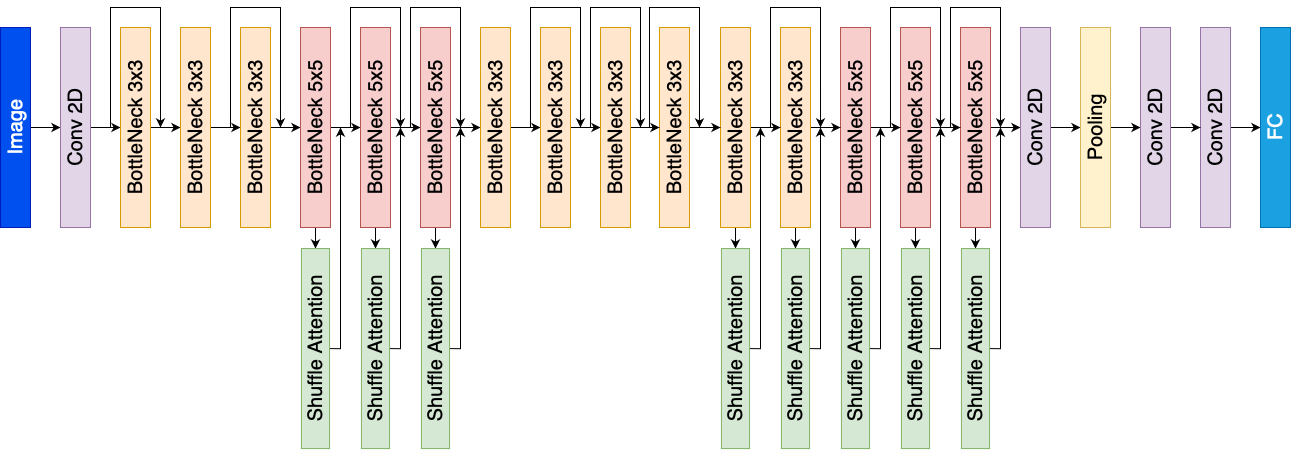
\includegraphics[width=1.0\textwidth]{image4-5}
  \caption{مدل پایه مبتنی بر لایه‌های كانولوشن و لایه توجه.}
  \label{image4-5}
\end{figure}

\noindent
در این معماری مسیر استخراج ویژگی از ۴ لایه كانولوشن، ۱ لایه رای گیری، ۱۵ لایه تنگنا \LTRfootnote{Bottleneck}  و ۸ ماژول توجه \LTRfootnote{Attention} تشکیل شده است، كه در ادامه توضیح داده خواهد شد. تصویر ورودی با ابعاد  $224 \times 224$  به بخش استخراج ویژگی داده می‌شود و مدل در این مسیر به طور خودكار یك سلسله مراتب ویژگی را از تصاویر ورودی آموزش خواهد دید و در نهایت این ویژگی‌های استخراج شده به عنوان ورودی دسته بند مورد استفاده قرار می‌گیرد.

\subsubsection{لایه كانولوشن}
۴ لایه کانولوشن دو بعدی همراه با گام \LTRfootnote{Stride}  یک یا دو استفاده شده است. در اولین لایه کانولوشن‌ اندازه پنجره فیلترها $3 \times 3$ و در لایه‌های کانولوشن بعدی اندازه پنجره فیلترها $1 \times 1$ می‌باشد. دلیل انتخاب سایز کوچک پنجره فیلترها کاهش پیچیدگی محاسباتی و همچنین عملکرد خوب آن‌ها در استخراج ویژگی می‌باشد. چگونگی عملکرد یک لایه کانولوشن از رابطه \ref{eq4-1} بدست می‌آید.

\begin{equation}	
x_j^{(l)} =\sum_{i=0}^{c} w_{c_{ij}}^{(l)}\ast x_i^{(l-1) }+ b_j^{(l)} 
\label{eq4-1}
\end{equation}

\noindent
که در آن $l$ نشان دهنده شماره لایه کانولوشن، $b$ و $w$ پارامترهای مدل، $x$ خروجی هر لایه $j\in[1,n]$ بیانگر شماره فیلتر موجود درلایه $l$ و همچنین $n$ بیانگر تعداد کل فیلترها در لایه $l$ و $\ast$ نشان دهنده عملگر کانولوشن می‌باشد.

\subsubsection{لایه تنگنا و واحد باقیمانده}
به عنوان مثال به جای پردازش یک نگاشت ویژگی عظیم با 256 عمق، ابتدا همه این اطلاعات را در نگاشت‌های ویژگی 64 بعدی فشرده می‌کنیم. زمانی که این فشردگی انجام شد، از کانولوشن 3×3 استفاده می‌کنیم که وقتی روی 64 نگاشت ویژگی به جای 256 نگاشت اعمال شود، بسیار سریع‌تر است و چنین پردازشی می‌تواند همان نتایج یا نتایج بهتری نسبت به پشته‌های معمولی 3×3 ارائه کند. در نهایت با استفاده از 1×1 مجدداً به نگاشت اصلی 256 خود بازمی‌گردیم.

\noindent
از سوی دیگر شبکه‌های عمیق با واحدهای باقیمانده\LTRfootnote{Deep Residual Network}  بر روی پایگاه داده‌های مختلف مانند \lr{ImageNet}  و COCO، دقت و همگرایی خوبی را از خود نشان داده‌اند. با استفاده از مسیرهای پرش\LTRfootnote{Shortcut Pathway}، واحدهای باقیمانده می‌توانند به سیگنال‌ها اجازه دهند که مستقیماً از یک بلوک به بلوک‌های دیگر منتقل شوند. به طور کلی، واحدهای باقیمانده را می‌توان به صورت رابطه \ref{eq4-2} بیان کرد.

\begin{equation}
x_{l+1}=x_l+R(x_l ,W_l)
\label{eq4-2}
\end{equation}

\noindent
در اینجا $R$ نشان دهنده تابع واحد باقیمانده است، $x_l$ ویژگی ورودی به واحد باقیمانده $l$ ام و $W_l$ مجموعه‌ای از پارامترهای مربوط به واحد باقیمانده $l$ام می‌باشد. ایده اصلی شبکه‌های باقیمانده، عمیق‌تر کردن یک شبکه به منظور افزایش دقت شبکه مورد نظر می‌باشد. بنابراین با این عملیات در واقع به شبکه اجازه داده می‌شود که در صورت نیاز، ویژگی‌های لایه قبل بدون تغییر و به صورت مستقیم به لایه بعد منتقل شود. در شکل \ref{image4-6} لایه تنگنا با واحد باقیمانده طراحی شده در این مدل به نمایش گذاشته شده است.

\begin{figure}[h]
\centering
  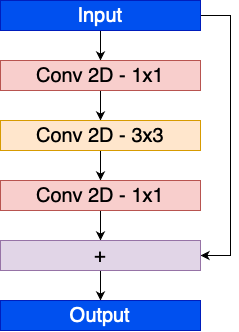
\includegraphics[width=0.25\textwidth]{image4-6}
  \caption{یک لایه تنگنا با واحد باقیمانده که با استفاده از کانولوشن های 1×1 اقدام به کاهش ابعاد نگاشت ویژگی می‌کند.}
  \label{image4-6}
\end{figure}

\subsubsection{واحد توجه}
لایه توجه استفاده شده در این پژوهش یک واحد توجه SA \LTRfootnote{Shuffle Attention} است که در مقاله \cite{yang2021sanet} معرفی شده است. این لایه ابتدا ابعاد کانال را به چندین ویژگی فرعی قبل از پردازش موازی آنها تقسیم می‌کند. سپس، برای هر زیر ویژگی از یک واحد Shuffle برای به تصویر کشیدن وابستگی های ویژگی در هر دو بعد مکانی و کانال استفاده می‌کند. پس از آن ، همه زیر ویژگی ها جمع می شوند و یک عملگر تغییر کانال برای امکان برقراری ارتباط اطلاعاتی بین ویژگی های فرعی مختلف به کار گرفته می شود. معماری این ماژول در شکل \ref{image2-33} آمده است. این لایه شامل دو بخش اصلی وابسته به کانال\LTRfootnote{Channel Attention Module}  و وابسته به موقعیت \LTRfootnote{Spacial Attention Module}  می‌باشد. 

\noindent
یک نقشه ویژگی \LTRfootnote{feature map} به نام $X$ با ابعاد $C \times H \times W$ که در آن $C$ و $H$ و $W$ به ترتیب عمق کانال، ارتفاع و عرض هستند، به عنوان ورودی واحد توجه در نظر گرفته می‌شود. ابتدا $X$ به $G$ گروه در طول کانال تقسیم می‌شود. رابطه \ref{eq4-3} این موضوع را نشان می‌دهد. سپس هر $X_k$ در طول کانال به دو نیم تقسیم شده و $X_{k1}$ و $X_{k2}$ را تشکیل می‌دهند. یکی از این دو زیر نقشه ویژگی  \LTRfootnote{sub feature map} برای توجه وابسته به کانال و دیگری برای توجه وابسته به موقعیت مورد استفاده قرار می‌گیرد. این عملیات توجه به مفهوم چه چیزی؟ و کجا؟ معنا می‌بخشد. 

\begin{equation}
X = [X_1, ..., X_G], X_k \in \mathbb{R}^{C/G \times H \times W}
\label{eq4-3}
\end{equation}

\noindent
برای اتصال صحیح ماژول واحد توجه به معماری \lr{MobileNetV3} مقدار $G$ را برابر ۴ در نظر گرفتیم.

\textbf{توجه  وابسته به کانال}: 
با بهره‌گیری از وابستگی‌های بین کانال‌ها، می‌توان بر ویژگی‌های وابسته، تأکید کرده و استخراج ویژگی‌های معانی خاص را بهبود بخشید. بنابراین در این پژوهش یک ماژول توجه وابسته به کانال ایجاد شده تا به طور واضح وابستگی بین کانال‌ها را مدل کند. ابتدا نقشه ویژگی $X_{k1}$ که از مرحله قبل بدست آمده است، توسط یک لایه پولینگ میانگین گیر سراسری \LTRfootnote{Global Averaging Pooling} به یک نقشه ویژگی $s$ با ابعاد $C/2G \times 1 \times 1$ تبدیل می‌شود. رابطه \ref{eq4-4} نشان دهنده چگونگی ایجاد بردار نقشه توجه وابسته به کانال می‌باشد. 

\begin{equation}
s = \frac{1}{H \times W}\sum_{i=1}^{H} \sum_{j=1}^{W} X_{k1} (i, j)
\label{eq4-4}
\end{equation}

\noindent
با انجام این عملیات، اطلاعات مکانی کلی برای هر کانال به صورت جداگانه محاسبه می‌شود و در $s$ قرار می‌گیرد. سپس خروجی لایه توجه وابسته به کانال مطابق رابطه \ref{eq4-5} بدست ‌می‌آید. 

\begin{equation}
X^{\prime}_{k1} = \sigma(W_1 s + b_1) . X_{k1}
\label{eq4-5}
\end{equation}

\noindent
که در آن $W_1\in R^{C/2G \times 1 \times 1} $  و  $b_1\in R^{C/2G \times 1 \times 1} $ به ترتیب نشان دهنده وزن و بایاس می‌باشند. ‌‌‌سپس نقشه توجه وابسته به کانال بدست آمده در نقشه ویژگی‌های ورودی ضرب شده و خروجی حاصل را ارائه می‌دهد.

\textbf{توجه وابسته به موقعیت}: 
وجود ویژگی‌های متمایز برای درک تصویر ورودی ضرروی می‌باشد، که این ویژگی‌ها می‌تواند در بازه بزرگی از تنوع قرار بگیرند. به منظور مدل سازی روابط مبتنی  بر روی ویژگی‌های محلی، ماژول توجه وابسته به موقعیت استفاده می‌شود. ابتدا ورودی $X_{k2}$ توسط یک عملگر GN \LTRfootnote{Group Norm} نرمال سازی می‌شود و خروجی این مرحله طبق رابطه \ref{eq4-6} بدست می‌آید.

\begin{equation}
X^{\prime}_{k2} = \sigma(W_2 GN(X_{k2}) + b_2) . X_{k2}
\label{eq4-6}
\end{equation}

\noindent
که در آن $W_2\in R^{C/2G \times 1 \times 1} $  و  $b_2\in R^{C/2G \times 1 \times 1} $ به ترتیب نشان دهنده وزن و بایاس می‌باشند. ‌‌‌سپس نقشه توجه وابسته به کانال بدست آمده در نقشه ویژگی‌های ورودی ضرب شده و خروجی حاصل را ارائه می‌دهد. در نهایت نقشه ویژگی های  $X^{\prime}_{k1}$ و $X^{\prime}_{k2}$ در کنار هم قرار گرفته و نقشه ویژگی 
$X^{\prime}_{k} \in \mathbb{R}^{C/G \times H \times W}$
بدست می‌آید. 

\textbf{تجمع}: 
پس از مراحل بالا، تمام زیر ویژگی‌های $X_k$ جمع می‌شوند و سرانجام یک عملگر مخلوط کننده کانال \LTRfootnote{channel shuffle} را برای ادغام اطلاعات گروه‌ها در طول بعد کانال به کار می‌بریم. خروجی نهایی واحد توجه به همان اندازه $X$ است که یکپارچه سازی SA با معماری‌های مدرن را آسان می‌‌کند ٖ\cite{yang2021sanet}.

\subsection{تابع ضرر}
یکی از چالش های اصلی در یادگیری ویژگی‌ها با استفاده از شبکه‌های عصبی پیچشی عمیق \lr{(DCNN)} \LTRfootnote{Deep convolutional neural network} برای شناسایی چهره در مقیاس بزرگ، طراحی تابع ضرر مناسب است که قدرت تفکیک را افزایش دهد. از آن‌جایی که ‌شبکه \lr{MobileNetV3} معماری بسیار سبک تری نسبت به معماری‌های شناخته شده دیگر که در فصل ۲ معرفی شدند، دارد؛ بنابراین استخراج ویژگی‌ها از چهره و دسته بندی تصاویر چهره با دقت بالا برای این شبکه بسیار دشوار است. همچنین در مواردی شباهت چهره افراد به یکدیگر ‌کار را از آن‌چه هست سخت‌تر خواهد کرد. تابع ضرر ArcFace \cite{deng2019arcface} کمک می‌کند ویژگی‌های استخراج شده که متعلق به دو دسته متفاوت هستند، فاصله بیشتری از هم داشته باشند و در مقابل ویژگی های استخراج شده برای دو تصویر از چهره یک فرد یکسان، فاصله کمتری از هم داشته باشند؛ این تابع ضرر که می‌توان آن را به راحتی با هزینه‌های محاسباتی ناچیز پیاده سازی کرد، به کاهش مشکلات ذکر شده کمک می‌نماید. رابطه نهایی تابع ضرر ArcFace به صورت \ref{eq3-16} می‌باشد.

\noindent 
در این تابع مقدار حاشیه m فقط برای زاویه مقدار مربوط به برچسب صحیح اعمال می‌شود و باقی مقادیر بردار دست نخورده باقی می‌مانند. از آنچا که در فاصله بین 0 تا $\pi$ هرچه زاویه $\theta$ افزایش پیدا کند، باعث می‌شود $cos(\theta)$ کاهش پیدا کند، بنابرین همگرایی شبکه با کندی مواجه خواهد شد. ما این مشکل را اصلاح کردیم و مقدار حاشیه m را به تمام مقادیر بردار خروجی اضافه می‌نماییم. تابع نهایی به صورت رابطه \ref{eq4-9} نوشته می‌شود.

\begin{equation}
L = - \frac{1}{N} \sum_{i=1}^{N} log \frac{e^{s(cos(\theta_{y_i}+m))}}{\sum_{j=1}^{n} e^{s(cos(\theta_j + m))}}
\label{eq4-9}
\end{equation}

\noindent 
حاصل ضرب وزن‌‌ها در ویژگی های استخراج شده محاسبه می‌گردد، که برابر $cos(\theta_j)$ می‌شود‌‌. سپس $arccos$ آن محاسبه شده که مقدار $\theta_j$ را به ما می‌دهد. سپس برای افزایش حاشیه بین $x_i$ و $W_j$ یک مقدار حاشیه زاویه‌ای $m$ به تمام زاویه‌ها اضافه می‌کنیم‌ تا به طور همزمان فشرده سازی درون کلاسی و اختلاف بین کلاسی را افزایش دهیم. در انتها دوباره $cos(\theta_j)$ محاسبه شده و در ثابت $s$ ضرب می‌شود.  مراحل بعدی دقیقاً مانند ArcFace هستند. در این روش بنا به پیشنهاد مقاله \cite{deng2019arcface} مقدار $m=0.5$ و مقدار $s=64$ در نظر گرفته شده است. مزایای این روش پیشنهادی را می‌توان به شرح زیر خلاصه کرد:

\begin{itemize}
 \item
در مجموعه داده‌های تصویر و فیلم در مقیاس بزرگ‌، به عملکرد مناسبی دست می‌یابد. زیرا ویژگی‌هایی که استخراج ‌می‌شود، علاوه بر اینکه قابل تفکیک \LTRfootnote{Separable} هستند، متمایز کننده \LTRfootnote{Discriminative} نیز هستند، و کمک می‌کند ویژگی‌های استخراج شده که متعلق به دو دسته متفاوت هستند، فاصله بیشتری از هم داشته باشند و در مقابل ویژگی‌های استخراج شده برای دو تصویر از چهره یک فرد یکسان، فاصله کمتری از هم داشته باشند.
 \item
فقط به چندین خط کد نیاز دارد و اجرای آن در چارچوب‌های \LTRfootnote{FrameWork} یادگیری عمیق مبتنی بر \lr{Pytorch} و \lr{Tensorflow} آسان است. برای داشتن عملکرد پایدار نیازی به ترکیب با سایر توابع ضرر ندارد و به راحتی همگرا می‌شود.
 \item
هنگام آموزش فقط پیچیدگی محاسباتی ناچیز را اضافه می‌کند. پردازنده های گرافیکی کنونی می‌توانند به راحتی از هزاران دسته مختلف برای آموزش پشتیبانی کنند و مدل به راحتی می‌تواند هویت‌های بیشتری را پشتیبانی کند.
\end{itemize} 

\subsection{آموزش مدل و استخراج ویژگی}
استفاده از روش پیشنهادی ما کمک می‌کند تا تعداد دسته ها پس از آموزش قابل تغییر باشد و همچنین برای یادگیری تک تصویری \LTRfootnote{one shot learning} بسیار مناسب است. در این بخش به آموزش روش پیشنهادی می‌پردازیم. مجموعه داده خود را پس از پیش‌پردازش و افزایش‌ داده‌ها \LTRfootnote{Data Augmentation}، آماده می‌کنیم. برای افزایش داده‌ها از چرخش افقی \LTRfootnote{Horizontal Flip} استفاده می‌کنیم. داده‌های آموزش متفاوت را بارگزاری کردیم و آموزش را در 30 دوره \LTRfootnote{Epoch} انجام داده‌ایم. در ابتدای روند آموزش، لازم است پارامترهای مدل مقدار دهی اولیه شوند. انتخاب پارامترهای اولیه میتواند تأثیر زیادی در مدل آموزش یافته داشته باشد. در این پژوهش به منظور مقدار دهی اولیه پارامترها از تابع توزیع یكنواخت استفاده شده است. 

\noindent
از دیگر چالش‌های اساسی برای روش‌های بهینه سازی مبتنی بر گرادیان، انتخاب میزان نرخ یادگیری مناسب است. روش‌های كلاسیك گرادیان تصادفی از نرخ یادگیری ثابت یا كاهشی استفاده میكنند، كه برای همه پارامترهای مدل یكسان است. با این حال، مشتقات جزئی پارامترهای لایه‌های مختلف می‌توانند از نظر مقدار متفاوت باشند، كه می‌تواند به نرخ یادگیری مختلفی نیاز داشته باشد. با این حال، مشتقات جزئی پارامترهای لایه‌های مختلف می‌توانند از نظر مقدار تفاوت قابل توجه‌ای داشته باشند، كه می‌تواند به نرخ یادگیری مختلفی نیاز داشته باشد. در سال‌های اخیر، تمایل به توسعه روش‌هایی برای انتخاب خودكار نرخ یادگیری مستقل افزایش یافته است. اكثر روش‌ها به عنوان مثال
RMSprop، 
AdaDelta، 
AdaGrad
و Adam آمارهای مختلف مشتقات جزئی را در چندین تكرار جمع آوری می‌كنند و از این اطلاعات برای تعیین میزان یادگیری سازگار برای هر پارامتر استفاده می‌كنند. این امر به ویژه برای آموزش شبكه‌های عمیق بسیار مهم است، جایی كه نرخ یادگیری مطلوب اغلب برای هر لایه بسیار متفاوت است. در این پژوهش در آزمایشات انجام شده از همه روش‌های نام برده استفاده شد ولی روش Adam عملكرد بهتری ارائه داده است.

\subsubsection{دسته‌بندی}
در مرحله آزمون به منظور تشخیص هویت یک تصویر چهره، پس از پیش‌پردازش تصویر را مطابق با ورودی شبکه تغییر اندازه می‌دهیم و جهت استخراج ویژگی‌ به آن شبکه می‌دهیم. پس از استخراج ویژگی‌ها توسط شبکه، بردار ویژگی ۵۱۲ تایی بدست آمده را با بردارهای مربوط به چهره های بانک اطلاعاتی مقایسه کرده و با محاسبه فاصله اقلیدسی بردارها، نزدیک ترین شخص مورد نظر انتخاب شده و در صورتی که فاصله میان بردار ویژگی آن‌ها از حد آستانه کمتر باشد، عمل دسته بندی انجام شده و هویت چهره مورد نظر تعیین می‌شود. در غیر این صورت اعلام می‌داریم که شخص مورد نظر قابل شناسایی نمی‌باشد.

\section{فناوری‌های استفاده شده}
پیاده‌سازی این الگوریتم به کمک زبان برنامه‌ نویسی پایتون و کتابخانه \lr{PyTorch} و \lr{OpenCV} انجام شده است. از کتابخانه‌های مهم مورد استفاده دیگر در این کار می‌‌توان به \lr{NumPy} برای انجام محاسبات ماتریسی و \lr{SciPy} و \lr{Scikit Learn} اشاره کرد. برای آموزش شبکه عصبی مربوط به دسته بندی ۱۲ گیگابایت حافظه اصلی و ۱۲ گیگابایت حافظه گرافیکی در اختیار گرفتیم.
